\documentclass{article}

\usepackage{geometry}
\usepackage{graphicx}
\usepackage{amsmath}

\title{Using seven segment LED display in multiplexing in EdSim -- an EMISY laboratory}
\author{Maciej Marcinkiewicz (300371)}
\date{11th May 2021}

\newgeometry{lmargin=3.2cm, rmargin=3.2cm, bmargin=2.5cm}

\begin{document}

\maketitle

\section{Introduction}
\subsection{Brief description}
Laboratory's main purpose was to learn how to handle 7-segment LED displays. The task
was to use 8051 microcontroller to display characters on 4 such displays. Everything
had to be done in EdSim5 simulator.

\subsection{Schematic}
\begin{figure}[h!] %possible: b, t, h, p and override (!)
    \centering
        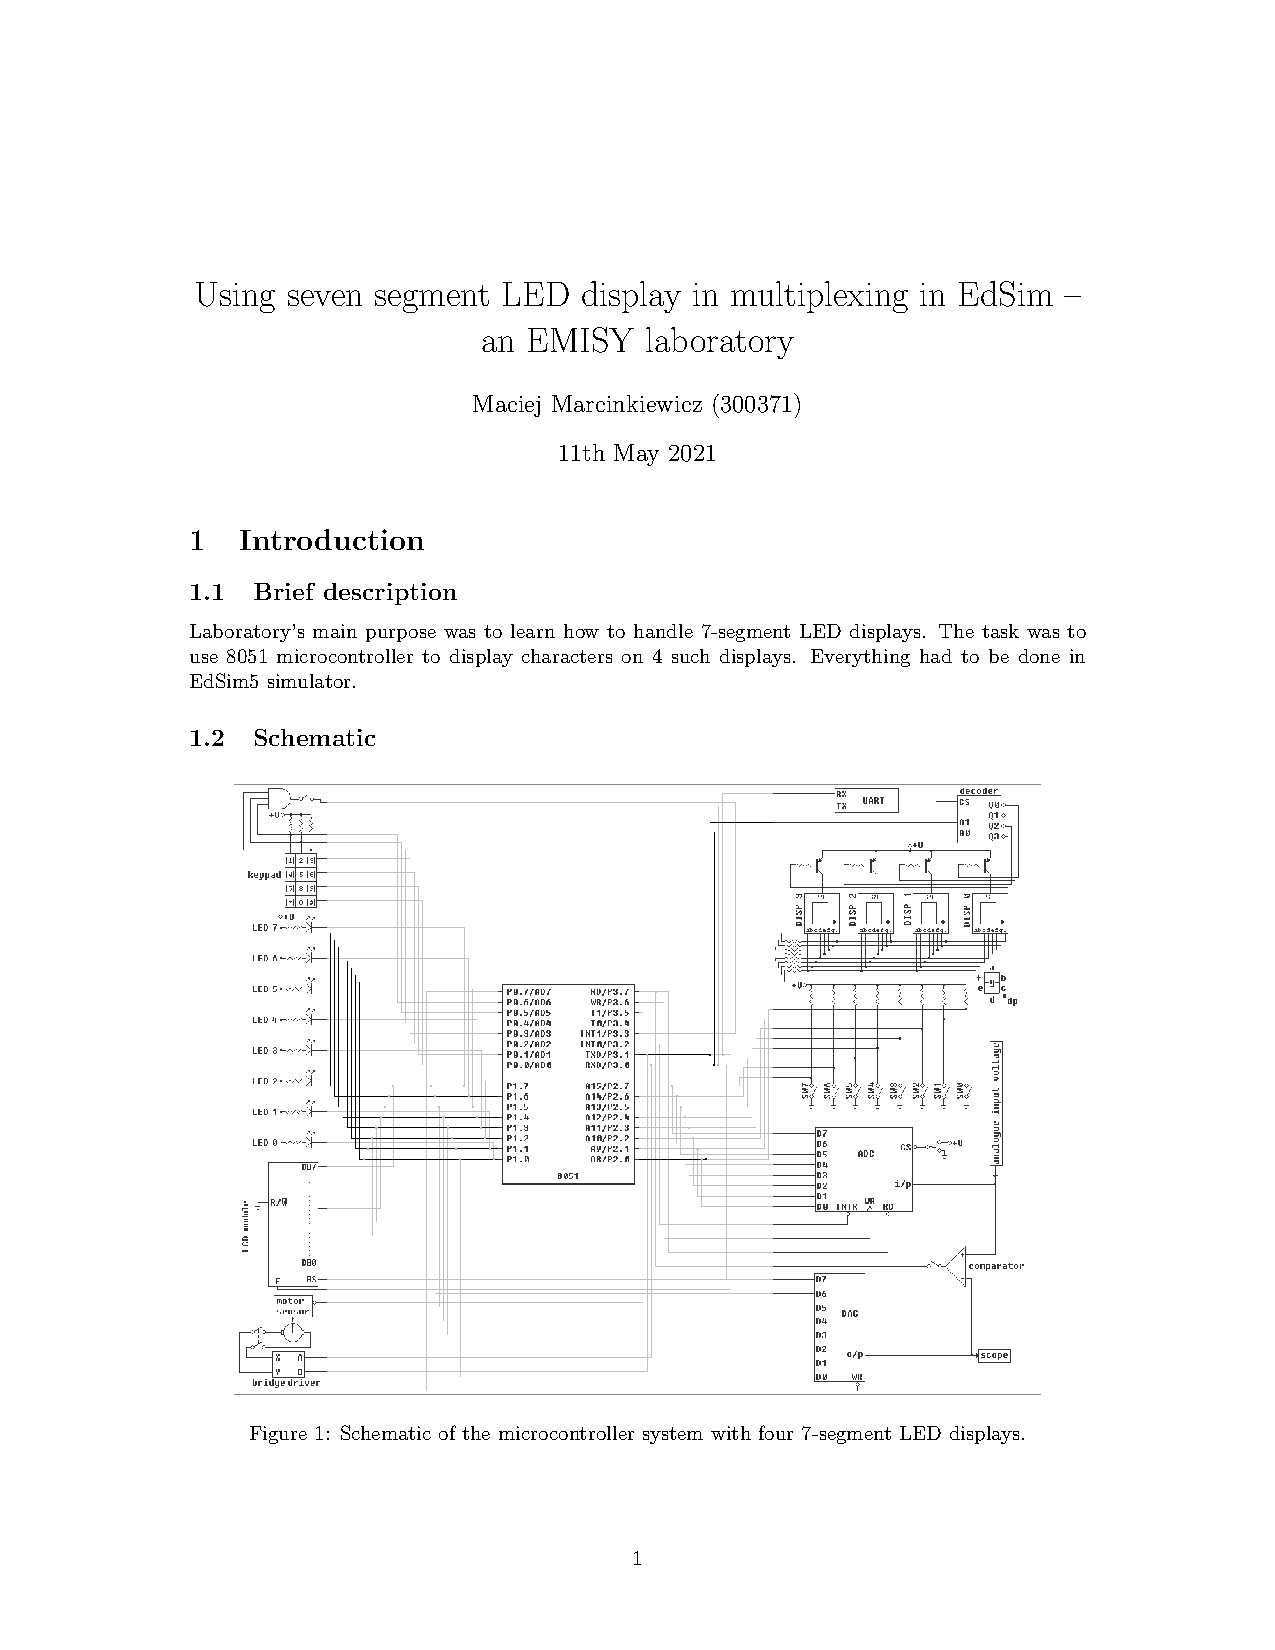
\includegraphics[width=0.9\linewidth]{lab2.png}
    \caption{Schematic of the microcontroller system with four 7-segment LED displays.}
\end{figure}

\subsection{Hardware description}
Microcontroller (Atmel's AT89C4051) is connected to 5 V source and is equipped with 12 MHz clock and 
simple resetting circuit. LED displays' cathodes are connected to P1 GPIO port. Common anodes
are connected to outputs of simple 2-address decoder. They are connected through inverters
and BJT transitors. Decoder's chip select pin is connected to P2.0 pin. Address pins
A0 and A1 are connected to P3.0 and P3.1 pins, respectively.

Decoder is used to select active LED display. Display's segments are turned on by
sinking selected segment's pins to GPIO. Displays have common anodes, so in order to
turn on a segment one has to clear corresponding pin, not set as it may appear more intuitive.

\section{Task 1}
\subsection{Assembly code}
\ttfamily
; define constants\\
; DISPLAY\_BUS is port to which cathodes of displays are connected\\
; DECODER\_CS is decoder's chip select pin\\
; DECODER\_ADDR decoder's (decoder) address pins; in fact only P3.0 and P3.1 are used\\
\\
DISPLAY\_BUS     equ     P1\\
DECODER\_CS      equ     P2.0\\
DECODER\_ADDR    equ     P3\\
\\
;-----------------------------start-----------------------------------\\
    mov     DISPLAY\_BUS, \#11111111b ; set all GPIO pins in P1 in order to turn off the display\\
\\
    mov     R0, \#2                  ; activate 3rd display\\
    mov     R1, \#10010010b          ; set pins to turn on segments which will show digit 5\\
    lcall   show\_digit              ; call function: R0 - active display; R1 - segments to display\\
\\
    jmp     \$                       ; infinite loop\\
\\
; subroutine which turns on selected segments in selected display\\
show\_digit:\\
    clr     DECODER\_CS          ; turn off the decoder\\
    mov     DECODER\_ADDR, R0    ; select active display with decoder\\
    mov     DISPLAY\_BUS, R1     ; set cathodes of display to turn on selected segments\\
    setb    DECODER\_CS          ; turn on decoder (ergo turn on display)\\
\\
    ret                          ; return from function

\subsection{Code description}
\rmfamily
Program starts with defining names for GPIO ports/pins in order to have clean and readable
code. In the beginning P1 port is written with 11111111$_2$ because 1 on each pin corresponds
to turned off segment. Later in this code program will set pins to 0 which will activate segments.

To make possible turning on any segments on any selected display, I have created show\_digit
subroutine. It requires to pass number of display (staring from 0) to the R0 register
and information about segments which will be turned on to the R1 register. In my case
I have selected display 2 and digit 5 to be shown.

Digit 5 is being displayed by turning on segments a, c, d, f and g. That is why
10010010$_2$ has been loaded to the R0 register. After passing parameters and calling the function
an endless loop has been set up to keep digit on the display.

Regarding show\_digit subroutine, it starts with CS pin clearing. It is done to make sure
that display will not show anything before setting up data. CS pin is responsible for
turning on decoder. When CS is cleared it ignores input data. Then address pins
of decoder are loaded with R0 value (first parameter of function) and bus for dislpay
(P1 port) is loader with R1 value (second parameter). The last step is turing on decoder
and return from function. Now display 2 should show digit 5.

\section{Task 2}
\subsection{Code}
\ttfamily
; define constants\\
; DISPLAY\_BUS is port to which cathodes of displays are connected\\
; DECODER\_CS is decoder's chip select pin\\
; DECODER\_ADDR decoder's (decoder) address pins; in fact only P3.0 and P3.1 are used\\
\\
DISPLAY\_BUS     equ     P1\\
DECODER\_CS      equ     P2.0\\
DECODER\_ADDR    equ     P3\\
\\
;-----------------------------start-----------------------------------\\
    mov     DISPLAY\_BUS, \#11111111b ; set all GPIO pins in P1 in order to turn off the display\\
    jmp     init\\
\\
    ; interrupt handler\\
    org     0Bh                         ; write instruction to 0xB address (interrupt handler)\\
\\
    clr     DECODER\_CS                  ; turn off the decoder\\
    mov     DECODER\_ADDR, \#3            ; select active display with decoder\\
    xrl     DISPLAY\_BUS, \#10000000b     ; use xor on display bus to change the most significant bit to make segment blinking\\
    setb    DECODER\_CS                  ; turn on decoder (ergo turn on display)\\
\\
    mov     TL0, \#0DFh                   ; restore timer\\
    mov     TH0, \#0B1h\\
\\
    reti\\
    \\
init:\\
; timer T0 configuration\\
    setb    TR0                 ; turn on T0 timer\\
    mov     TMOD, \#00000001b    ; set mode 1, count internal clock cycles, do not react in external interrupts\\
    setb    ET0                 ; enable overflow interrupt\\
    setb    EA                  ; enable global interrupt\\
\\
    mov     TH0, \#0B1h\\
    mov     TL0, \#0DFh           ; load timer with 0xFFFF - 20000 in order to set timer to 20 ms\\
\\
    jmp     \$

\rmfamily
\subsection{Code description}
In the beginning all P1 port's pins are set to make sure that displays are in initial state.
After that being done, program jumps to init section where timer is initialized. TR0 bit is set
to turn on T0 timer. Then program loads 00000001$_2$ to TMOD register. Only lower half of that register
concerns T0 timer. Two least significant bits are responsible for selecting mode. 01$_2$ sets mode 1, 
a 16-bit mode (i.e. both TH0 and TL0 registers work as 8-bit regsiters). Two most significant bits of this nibble
are responsible for not reacting on external interrupts and counting internal clock cycles.

The last settings are ET0 and EA bits of TCON register (both bits are set). They enablr overflow interrupt and
global interrupt, respectively. When configuration is being done, program loads TH0 register with B1$_{16}$
and TL0 with DF$_{16}$. The task was to wait 20 ms between each switching on/off the segment, so timer's registers
have to be loaded with FFFF$_{16}$ - 20000$_{10}$ which is equal to DFB1$_{16}$. Timer increments value in each machine cycle
and when overflow happens interrupt is being sent and then handled. Because of that maximal possible value has to be
substracted by 20000 -- length of delay in microseconds -- to get proper starting value.

From that moment timer starts to work and program stays at loop until interrupt happens. When it happens, program jumps
to 0xB in memory to execute handler's code. Sequence of turing on segment is the same as previously, so it does not need
further clarification. However, this time segment has to blink, so pin's state has to change into opposite one with each
timer's cycle. For that purpose logical XOR function may be used -- in this case the most significant bit (decimal point segment) is changing state
with each handler execution. In the end timer is being restored and program returns to the infinite loop.

\section{Task 3}
\subsection{Code}
\ttfamily
; define constants\\
; DISPLAY\_BUS is port to which cathodes of displays are connected\\
; DECODER\_CS is decoder's chip select pin\\
; DECODER\_ADDR decoder's (decoder) address pins; in fact only P3.0 and P3.1 are used\\
\\
DISPLAY\_BUS     equ     P1\\
DECODER\_CS      equ     P2.0\\
DECODER\_ADDR    equ     P3\\
\\
    jmp     init                ; jump to initialization of the timer\\
\\
    ; interrupt handler\\
    org     0Bh                 ; write instruction to 0xB address (interrupt handler)\\
\\
    mov     ACC, R0             ; read indicator of which display should be turned on\\
    jb      ACC.0, display0     ; go to display 0\\
    jb      ACC.1, display1     ; go to display 1\\
    jb      ACC.2, display2     ; go to display 2\\
    jb      ACC.3, display3     ; go to display 3\\
\\
display0:\\
    mov     R0, \#00000010b      ; set indicator for display 1\\
    \\
    mov     R1, \#0              \\
    mov     R2, \#11111001b\\
    lcall   show\_digit          ; call show\_digit to display number 1 on display 0\\
    \\
    mov     TL0, \#0DFh          ; restore timer\\
    mov     TH0, \#0B1h\\
\\
    reti\\
\\
display1:\\
    mov     R0, \#00000100b      ; set indicator for display 2\\
\\
    mov     R1, \#1\\
    mov     R2, \#11111000b      \\
    lcall   show\_digit          ; call show\_digit to display number 7 on display 1\\
    \\
    mov     TL0, \#0DFh          ; restore timer\\
    mov     TH0, \#0B1h\\
\\
    reti\\
\\
display2:\\
    mov     R0, \#00001000b      ; set indicator for display 3\\
\\
    mov     R1, \#2\\
    mov     R2, \#11111001b\\
    lcall   show\_digit          ; call show\_digit to display number 1 on display 2\\
    \\
    mov     TL0, \#0DFh          ; restore timer\\
    mov     TH0, \#0B1h\\
\\
    reti\\
\\
display3:\\
    mov     R0, \#00000001b      ; set indicator for display 0\\
\\
    mov     R1, \#3\\
    mov     R2, \#11000000b\\
    lcall   show\_digit          ; call show\_digit to display number 0 on display 3\\
    \\
    mov     TL0, \#0DFh          ; restore timer\\
    mov     TH0, \#0B1h\\
\\
    reti\\
\\
init:\\
    mov     DISPLAY\_BUS, \#11111111b ; set all GPIO pins in P1 in order to turn off the display\\
; timer T0 configuration\\
    setb    TR0                 ; turn on T0 timer\\
    mov     TMOD, \#00000001b    ; set mode 1, count internal clock cycles, do not react in external interrupts\\
    setb    ET0                 ; enable overflow interrupt\\
    setb    EA                  ; enable global interrupt\\
\\
    mov     TH0, \#0B1h\\
    mov     TL0, \#0DFh          ; load timer with 0xFFFF - 20000 in order to set timer to 20 ms\\
\\
    mov     R0, \#00000001b      ; set indicator for display 0\\
\\
    jmp     \$\\
\\
; subroutine which turns on selected segments in selected display\\
show\_digit:\\
    clr     DECODER\_CS          ; turn off the decoder\\
    mov     DECODER\_ADDR, R1    ; select active display with decoder\\
    mov     DISPLAY\_BUS, R2     ; set cathodes of display to turn on selected segments\\
    setb    DECODER\_CS          ; turn on decoder (ergo turn on display)\\
\\
    ret                         ; return from function

\rmfamily

\newpage

\subsection{Code description}
The last task was to display last 4 digits of student's album number (0171) with multiplexing animation.
Program consist of initialization part (the same as in the previous task), displaying digit subroutine, interrupt handler and 
four subroutines responsible for displaying a digit in a specified display. Selection of display works
in the way, that R0 register contains an indicator of what display should be turned on next time.

For instance, 00000100$_2$ means that display 2 has to be turned on next time. Handler loads accumulator
with R0 content because it can be accessed by bit. Program jumps to the proper subroutine, sets new indicator for next display, shows a digit,
restores the timer and returns to the infinite loop where program waits for the next interrupt.

In that way program displays digits in a sequence display 0 - display 1 - display 2 - display 3 (1-7-1-0).

\section{Final questions}
\subsection*{Describe how is a display selected in EDSIM simulator?}
Display is selected through decoder. Microcontroller provides information to the address
pins, decoder turns on proper output pin. Selected pin activates BJT switch and in this
way provides voltage to the common anode of the display.

\subsection*{What is the difference between common anode and common cathode LED displays in terms of interfacing them with MCU?}
As it was described in the introduction, common anode dislpay requires to clear bits
corresponding to the segments' cathodes to turn on selected segments. In common
cathode LED display it has to be done in the opposite way -- to turn on segment GPIO pin
have to provide voltage.

\subsection*{How can be a timer peripheral used to generate precise time intervals (precise delays)?}
Timer's registers can be loaded with value of FFFF$_{16}$ - desired delay in microseconds (in the case
of 12 MHz clock) and overflow may be used as an interrupt signal. Timer increments value in
register with each machine cycle, so flag will be raised after the amount of time we desired.

\subsection*{How does multiplexing driving mode of LED displays work? Compare it with static driving mode of LED displays in terms 
of required GPIO pins and current consumption. When does it make sense to use multiplexing and when does it not?}
In multiplexing driving mode microcontroller turns on displays in a sequence with such small delays
that it is barely visible for eye and creates an illusion of a static image. For us it is
not a problem, however taking a photo of such display will reveal how this technique works
and displayed characters will not appear in the photo in proper way. This wil not happen
when LED displays are driven staticly. However this technique requires more pins and more
current as microcontroller has to provide it constantly.

\section*{Declaration of authorship}
I declare that this piece of work which is the basis for recognition of achieving learning outcomes in the EMISY course was completed on my own.

\end{document}